% IEEEtran conference draft generated by paper/build_paper.py. Compile with: pdflatex, pdflatex.
\documentclass[conference]{IEEEtran}
\usepackage{amsmath,amssymb,graphicx,booktabs,cite}
\usepackage[T1]{fontenc}
\begin{document}
\title{Source-Grounded Verification of Large Language Model Answers: A Browser-Based System and a Cross-Model Audit Protocol}
\author{
\IEEEauthorblockN{Piush Kole}
\IEEEauthorblockA{Department of Computer Science\\ Christ University\\ {piushkole@msds.christuniversity.in}}
\and
\IEEEauthorblockN{Thrilok M}
\IEEEauthorblockA{Department of Computer Science\\ Christ University\\ {thrilok.m@msds.christuniversity.in}}
}
\maketitle

\begin{abstract}
Large language models (LLMs) produce fluent answers that readers rarely verify. We present Synthetic Silence, a browser extension and local service that splits text into factual claims, retrieves sources from Wikipedia and OpenAlex, assesses what each source says about each claim, and returns one of five verdicts (supported, refuted, mixed, insufficient, or no sources) together with the quoted passage that justifies it. The verdict follows deterministic rules over per-source stances. A density-based representation-space signal studied in earlier work is kept only as an experimental indicator, because it did not generalise across constructions. On 100 balanced FEVER claims, Wikipedia retrieval raised accuracy on SUPPORTS and REFUTES claims from 66.7\% to 79.7\% over scholarly-only retrieval (paired exact test p = 0.06, suggestive only), but a pooled natural-language-inference score never abstained (0\% recall on NOT ENOUGH INFO). A per-source stance variant recovered abstention (61.3\% recall) at significantly lower accuracy on decisive claims (49.3\%, p < 0.001 against the pooled score). We also specify a cross-model audit that compares the share of each LLM's claims that sources back up or push against under one fixed checker. The audit's results are not part of this draft.
\end{abstract}

\begin{IEEEkeywords}
fact-checking, large language models, hallucination, retrieval, natural language inference, evidence sufficiency, browser extension
\end{IEEEkeywords}

\section{Introduction}
People now read answers written by language models in the same place they read everything else: inside a web browser. The answers are fluent and specific, and a specific falsehood reads exactly like a specific fact. Surveys of generation research document that models state unsupported or contradicted content with confidence \cite{ji2023}, and benchmarks such as TruthfulQA show that larger models can reproduce common human misconceptions more often, not less \cite{lin2022}.

Automated fact-checking offers a remedy, but most published systems are built for benchmark claims that arrive already isolated, with a fixed evidence corpus \cite{guo2022,thorne2018}. A reader of a paragraph has neither. The paragraph must be split into checkable claims, evidence must be found for each, and the result must be shown at the moment of reading, with a way to inspect the sources. A further difficulty is that a missing source and a failed search look the same to the user unless the system keeps them apart.

This paper makes four contributions.

\begin{itemize}
\item A claim-level verification pipeline and Chrome extension that return a five-valued verdict with a verbatim supporting quote per source (Section III).
\item A verdict rule set that is deterministic and auditable: given per-source stances it needs no further model call (Section III-E).
\item An explicit treatment of failure: a retrieval outage, a spent search budget and a model error are reported as errors for the affected claim and are never presented as the absence of evidence (Section III-H).
\item A validation on FEVER \cite{thorne2018} with confidence intervals, an analysis of the failure of a first per-source variant, and a protocol for auditing several LLMs under one fixed checker (Sections IV and V).
\end{itemize}

The work continues an earlier study of whether representation-space density signals evidence insufficiency \cite{ss2026}. That study found the signal weak on FEVER (AUROC 0.5463), inverted on AVeriTeC (AUROC 0.2754) and at chance under a change of reference manifold. We therefore do not use density to decide the verdict; the system reports it separately and labels it experimental.

\section{Related Work}
\subsection{Automated fact-checking}

Guo et al. survey the task as claim detection, evidence retrieval, verdict prediction and justification production \cite{guo2022}. FEVER pairs Wikipedia-derived claims with the labels SUPPORTS, REFUTES and NOT ENOUGH INFO \cite{thorne2018}. AVeriTeC moves to real-world claims with evidence from the open web \cite{schlichtkrull2023}. Our validation uses FEVER because its labels let us measure abstention directly; we discuss in Section VI why its Wikipedia origin limits what the numbers show.

\subsection{Hallucination detection and factuality of generated text}

SelfCheckGPT detects hallucinated sentences by sampling the same model several times and measuring consistency, without external evidence \cite{manakul2023}. FActScore decomposes a long generation into atomic facts and reports the share supported by a knowledge source \cite{min2023}. Our cross-model audit is close in spirit to FActScore, but it checks claims with a retrieval pipeline that runs in the reader's browser rather than against a fixed biography corpus.

\subsection{Density, distance and calibration}

Distance to a reference set is a common out-of-distribution score. We use cosine k-nearest-neighbour distance and Mahalanobis distance \cite{mahalanobis1936} with a Ledoit-Wolf shrunk covariance \cite{ledoit2004} over sentence embeddings \cite{reimers2019,wang2020}. Split-conformal prediction supplies a distribution-free way to turn a score into a calibrated decision \cite{angelopoulos2021}; our deployment carries that interface but does not fit it, and reports every score as uncalibrated.

\subsection{LLM judges}

Using one model to judge another is now common and has known biases, including a preference for answers from the same family \cite{zheng2023}. Our checker is held fixed across the audited models, which removes a difference between them caused by the checker but not a bias of the checker itself.

\section{System Design}
\subsection{Overview}

Fig. 1 shows the pipeline. A selected passage enters the extension, which sends it to a service running on the user's machine. The service extracts claims, retrieves and ranks sources, assesses each source's stance, and streams one result per claim back to the interface as soon as it finishes. Embedding and density computations run locally; language-model calls go to a hosted model through one provider interface.

\begin{figure}[t]
\centering
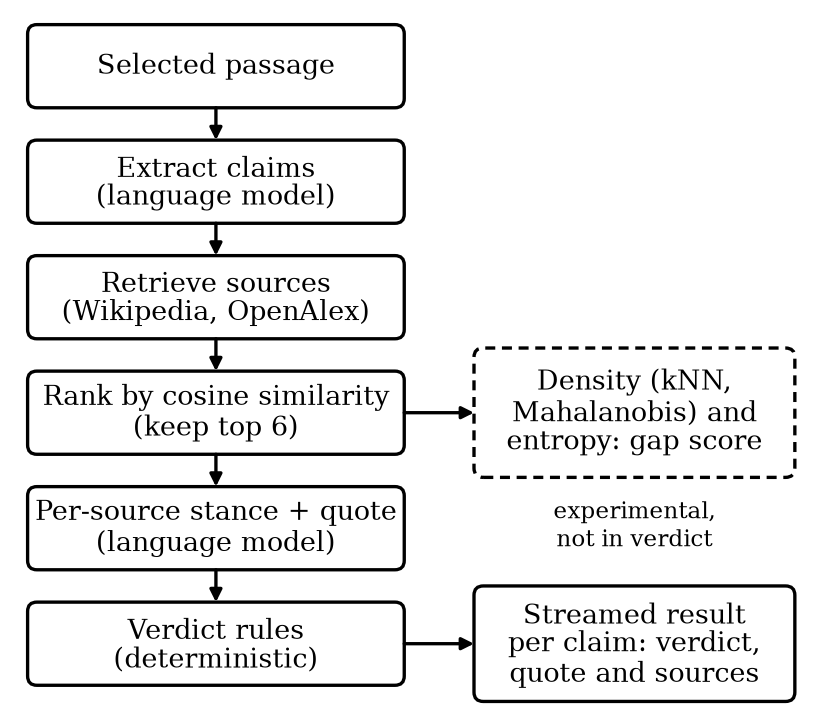
\includegraphics[width=\columnwidth]{figs/pipeline.png}
\caption{System overview. Solid boxes decide the verdict. The dashed box is computed alongside it and is shown only in research mode.}
\end{figure}

\subsection{Claim extraction and normalisation}

A language model returns the checkable factual assertions in the passage as self-contained statements, keeping names, numbers and dates as written and skipping opinions, questions and predictions. Duplicates are removed and identifiers are reassigned by the service rather than trusted from the model. The number of claims per request is capped (default six) and the response records whether the cap truncated the list. A second call produces a normalised form with a core entity and predicate. The normalised form is used only to build search queries. Stance and ranking use the claim exactly as written, because normalisation can drop the detail that makes a claim false.

\subsection{Retrieval}

Two retrievers run concurrently for each claim. The Wikipedia retriever issues two MediaWiki searches (the normalised sentence and the core entity) and keeps lead-section extracts of at most 1,000 characters. The OpenAlex retriever \cite{priem2022} searches scholarly works and reconstructs the abstract from its inverted index. Results are merged and deduplicated by identifier and by text. If a retriever fails while the other returns sources, the claim proceeds. If every retriever failed, or one failed and none returned anything, the claim fails with an error rather than returning an empty source list.

\subsection{Ranking}

Let $\mathbf{u}_c$ and $\mathbf{u}_{e_i}$ be sentence embeddings of the claim and of source $e_i$. Sources are ordered by cosine similarity

\begin{equation}
s_i = \cos(\mathbf{u}_c,\mathbf{u}_{e_i}) = \frac{\mathbf{u}_c \cdot \mathbf{u}_{e_i}}{\lVert \mathbf{u}_c \rVert\, \lVert \mathbf{u}_{e_i} \rVert}
\end{equation}

The top $K=6$ are kept. A source below the floor $s_i < 0.15$ is dropped only if it ranks below the first two, so a poor embedding match alone can never empty the list, which downstream would read as the absence of sources.

\subsection{Stance and verdict}

A single model call returns, for every kept source $i$, a stance $\sigma_i \in \{\text{supports},\text{refutes},\text{neutral},\text{irrelevant}\}$, a confidence $\kappa_i \in [0,1]$ and a quote $q_i$ copied from the source. The prompt requires every specific detail of the claim (names, dates, places, numbers and categories) to be confirmed for support, and treats a different year or category as a conflict. A stance of supports or refutes is kept only if $q_i$ is found verbatim in the source text after whitespace and case normalisation; otherwise it is downgraded to neutral. The counted sets are

\begin{equation}
\begin{aligned}
\mathcal{P} = \{\, i : \sigma_i = \text{supports},\ \kappa_i \ge 0.5,\ q_i \ne \emptyset \,\}, \\
\mathcal{N} = \{\, i : \sigma_i = \text{refutes},\ \kappa_i \ge 0.5,\ q_i \ne \emptyset \,\}
\end{aligned}
\end{equation}

A set qualifies to decide the verdict when it has two members, or one member of high confidence:

\begin{equation}
Q(S) = \bigl(|S| \ge 2\bigr) \lor \bigl(|S| = 1 \land \max_{i \in S} \kappa_i \ge 0.8\bigr)
\end{equation}

The verdict $v$ is the first rule that applies:

\begin{itemize}
\item no sources, if no source was retrieved;
\item mixed, if $\mathcal{P} \ne \emptyset$ and $\mathcal{N} \ne \emptyset$ and $Q(\mathcal{P}) \lor Q(\mathcal{N})$;
\item supported, if $Q(\mathcal{P})$; refuted, if $Q(\mathcal{N})$;
\item insufficient otherwise. If only one side has counted sources, the result is marked as leaning towards that side.
\end{itemize}

For display, let $\mathcal{R}$ be the sources whose stance is not irrelevant. The confidence-weighted support and conflict shares are

\begin{equation}
\begin{aligned}
\mathrm{supp} = \frac{\sum_{i \in \mathcal{R},\, \sigma_i = \text{supports}} \kappa_i}{\sum_{i \in \mathcal{R}} \kappa_i}, \\
\mathrm{conf} = \frac{\sum_{i \in \mathcal{R},\, \sigma_i = \text{refutes}} \kappa_i}{\sum_{i \in \mathcal{R}} \kappa_i}
\end{aligned}
\end{equation}

Worked example. Four sources return (supports, 0.95), (supports, 0.90), (neutral, 0.70) and (irrelevant, 0.90), each supporting quote verified. Then $\mathcal{P}=\{1,2\}$ and $Q(\mathcal{P})$ holds, so $v$ = supported. With $\mathcal{R}=\{1,2,3\}$, $\mathrm{supp} = (0.95+0.90)/(0.95+0.90+0.70) = 0.725$ and $\mathrm{conf}=0$.

A pooled alternative, used as the baseline, sends all sources in one call and obtains one entailment score $e$ and one contradiction score $c$. It returns refuted if $c \ge 0.5$, supported if $e \ge 0.6$, and insufficient otherwise. These are display bins, not calibrated thresholds.

\subsection{Experimental representation-space signals}

Two signals from the earlier study are computed for every claim. Embeddings are 384-dimensional all-MiniLM-L6-v2 vectors \cite{reimers2019,wang2020}. Let $\mathbf{q}$ be the claim embedding and $\mathbf{r}_{(1)},\dots,\mathbf{r}_{(k)}$ its $k=5$ nearest neighbours in a reference manifold of 10,000 FEVER claim embeddings. The neighbourhood distance is

\begin{equation}
d_k(\mathbf{q}) = \frac{1}{k}\sum_{j=1}^{k}\bigl(1-\cos(\mathbf{q},\mathbf{r}_{(j)})\bigr)
\end{equation}

and the Mahalanobis distance uses a Ledoit-Wolf shrunk covariance of the reference set:

\begin{equation}
\begin{aligned}
d_M(\mathbf{q}) = \sqrt{(\mathbf{q}-\boldsymbol{\mu})^{\top}\hat{\Sigma}^{-1}(\mathbf{q}-\boldsymbol{\mu})}, \\
\hat{\Sigma} = (1-\delta)\,S + \delta\,\frac{\operatorname{tr}(S)}{p}\,I
\end{aligned}
\end{equation}

The density score combines them, normalising $d_M$ by the maximum over the query batch $B$:

\begin{equation}
\rho(\mathbf{q}) = \frac{1}{2}\left(d_k(\mathbf{q}) + \frac{d_M(\mathbf{q})}{\max_{\mathbf{q}' \in B} d_M(\mathbf{q}') + \varepsilon}\right)
\end{equation}

This normalisation has a consequence that is easy to miss. When claims are scored one at a time, as in the earlier experiments and in this system, $|B|=1$ and the second term equals $d_M/(d_M+\varepsilon) \approx 1$ for every claim. The score reduces to $\rho \approx (d_k+1)/2$ and the Mahalanobis term carries no information. We keep the estimator unchanged so that the served score is the one that was evaluated.

The second signal is the normalised entropy of a softmax over claim-source similarities $s_1,\dots,s_N$ with temperature $\tau = 0.1$:

\begin{equation}
\begin{aligned}
p_i = \frac{\exp(s_i/\tau)}{\sum_{j=1}^{N}\exp(s_j/\tau)}, \\
U = -\frac{1}{\log N}\sum_{i=1}^{N} p_i \log p_i
\end{aligned}
\end{equation}

with $U=1$ when $N=0$ and $U=0$ when $N=1$. The experimental gap score is $G = (\rho + U)/2$, and a temporal feature $T = |\{i : y_i \ge y_0\}|/N$ is the share of sources published in or after a cutoff year $y_0$ (2023 by default; sources without a year count as earlier).

Worked example. For similarities $(0.62, 0.58, 0.31, 0.12)$ the softmax gives $p \approx (0.581, 0.389, 0.026, 0.004)$, so $H \approx 0.800$ and $U = 0.800/\ln 4 \approx 0.577$. With $d_k = 0.62$, $\rho = (0.62+1)/2 = 0.81$ and $G = (0.81+0.577)/2 \approx 0.694$.

Note that $U$ is high precisely when many sources match the claim about equally well, which is the case for a well-documented claim. A high $G$ can therefore accompany a well-supported claim, and this is why $G$ takes no part in the verdict (Section V-B).

\subsection{Calibration status}

A split-conformal calibrator \cite{angelopoulos2021} is available. For $n$ held-out scores $\{s_i\}$ and error level $\alpha$ it uses the threshold

\begin{equation}
\hat{q} = \operatorname{Quantile}\!\left(\{s_i\}_{i=1}^{n};\ \frac{\lceil (n+1)(1-\alpha) \rceil}{n}\right)
\end{equation}

For example $n=100$ and $\alpha=0.1$ give the level $0.91$. No calibration set exists for deployment, so the calibrator is never fitted and every signal carries the status NOT\_CALIBRATED.

\subsection{Failure semantics, streaming and privacy}

Results are streamed as newline-delimited JSON: the extracted claims first, then one event per claim, then a terminal event. A claim that fails produces an error event for that claim only; the others complete. A connection that closes without the terminal event is reported as an error and marks unfinished claims as failed, so an interrupted run cannot look complete. Finished claims are cached on disk under a key that includes the model, retrievers and prompt version; failures are never cached. Claim text is sent to the hosted language model, and search terms are sent to Wikipedia and OpenAlex. The interface states this, and the extension contacts only a loopback address for the backend.

\section{Evaluation Protocol}
\subsection{Verdict validation on FEVER}

We sample claims from the FEVER paper development split, balanced over SUPPORTS, REFUTES and NOT ENOUGH INFO (seed 42) and deduplicated by claim identifier. A verdict maps to a label as supported $\to$ SUPPORTS, refuted $\to$ REFUTES, and insufficient or no sources $\to$ NOT ENOUGH INFO; mixed is counted as wrong and reported separately. With $n$ scored claims and $n_c$ gold claims of class $c$, we report

\begin{equation}
\begin{aligned}
\mathrm{Acc} = \frac{1}{n}\sum_{k=1}^{n}\mathbb{1}[\hat{y}_k = y_k], \\
F1_c = \frac{2P_cR_c}{P_c+R_c}, \\
\text{macro-}F1 = \frac{1}{3}\sum_{c} F1_c
\end{aligned}
\end{equation}

and the accuracy restricted to SUPPORTS and REFUTES claims (decisive accuracy). Every proportion carries a 95\% Wilson interval \cite{wilson1927}:

\begin{equation}
\begin{aligned}
\frac{\hat{p} + \dfrac{z^2}{2n} \pm z\sqrt{\dfrac{\hat{p}(1-\hat{p})}{n} + \dfrac{z^2}{4n^2}}}{1 + \dfrac{z^2}{n}}, \\
z = 1.96
\end{aligned}
\end{equation}

The compared variants are run on the same claims. Claims whose run failed for an infrastructure reason are excluded from every variant, not just from the one that failed.

\subsection{Cross-model audit}

A fixed list of 40 prompts covers five domains (science, history, geography, medicine and technology) and eight common-misconception questions. Each model answers every prompt at temperature zero with the same system prompt, in three to five sentences. The planned models are GPT-4o (OpenAI), Claude Sonnet 4.5 (Anthropic), Gemini 2.5 Pro and Gemini 2.5 Flash (Google), Llama 3.3 70B (Meta), DeepSeek Chat (DeepSeek) and Mistral Large (Mistral AI), all reached through one API gateway; the exact model versions are recorded in the run metadata. API models can differ from the consumer chat products that share their names. Each answer is split into claims and each claim is checked by the same pipeline with the same checker model and retrievers. For a model $m$ with claim set $\mathcal{C}_m$ and verdict $v(c)$, the claim-level rate of a verdict $x$ is

\begin{equation}
R_m^{(x)} = \frac{\bigl|\{\, c \in \mathcal{C}_m : v(c) = x \,\}\bigr|}{|\mathcal{C}_m|}
\end{equation}

and the share of answers containing at least one refuted claim is

\begin{equation}
A_m = \frac{1}{|\mathcal{P}|}\sum_{p \in \mathcal{P}} \mathbb{1}\bigl[\exists\, c \in \mathcal{C}_{m,p} : v(c) = \text{refuted}\bigr]
\end{equation}

Claims within one answer are not independent, so the difference $\Delta = R_a^{(x)} - R_b^{(x)}$ between two models is given with a paired bootstrap interval \cite{efron1979} that resamples prompts, not claims. A failed model call or check is counted and reported, never scored as a verdict.

\subsection{Threats to validity}

\begin{itemize}
\item A refuted claim is one that retrieved sources push against. It is evidence about the source pool and the checker, not a ground-truth label.
\item The checker is a language model and may favour answers from its own family \cite{zheng2023}.
\item FEVER claims come from Wikipedia and may be known to the models; only relative comparisons between variants are meaningful.
\item NOT ENOUGH INFO means the dataset's annotators found no evidence in their corpus. It is not the same as the retrievers finding no source.
\item With about one hundred claims, intervals are roughly $\pm$10 percentage points.
\end{itemize}

\section{Results}
\subsection{Verdict validation on FEVER}

Table I compares three variants on the same 100 claims. The baseline run covered 150 sampled claims, but 50 failed because the anonymous OpenAlex request budget was exhausted; the other variants were run on the 100 claims the baseline scored. Of those, 69 are SUPPORTS or REFUTES, which is the denominator of decisive accuracy.

\begin{table}[t]
\caption{Verdict validation on 100 FEVER claims (same claims in every row)}
\centering
\footnotesize
\begin{tabular}{lcccc}
\toprule
Variant & Acc. (95\% CI) & Macro-F1 & Decisive acc. (95\% CI) & NEI recall \\
\midrule
Pooled, OpenAlex (baseline) & \shortstack{51.0\\(41.3--60.6)} & 0.466 & \shortstack{66.7\\(54.9--76.6)} & 16.1 \\
Pooled, Wikipedia & \shortstack{55.0\\(45.2--64.4)} & 0.445 & \shortstack{79.7\\(68.8--87.5)} & 0.0 \\
Stance, Wikipedia (first prompt) & \shortstack{53.0\\(43.3--62.5)} & 0.528 & \shortstack{49.3\\(37.8--60.8)} & 61.3 \\
\bottomrule
\end{tabular}
\par\vspace{2pt}{\scriptsize Percent, except macro-F1. NEI: NOT ENOUGH INFO. Coverage (claims with at least one relevant source) was 97.0, 100.0 and 95.0 percent in the three rows.}
\end{table}

Three observations follow. First, Wikipedia retrieval raises decisive accuracy over scholarly-only retrieval (66.7\% to 79.7\%), as expected for claims that were themselves written from Wikipedia. On the 69 decisive claims the pooled-Wikipedia variant was right and the baseline wrong on 14, and the reverse on 5; an exact paired test gives $p = 0.064$ and a paired bootstrap interval for the difference of $+1.4$ to $+24.6$ points, so the gain is suggestive rather than conclusive. Second, the pooled score never abstains: it labelled 25 of 31 NOT ENOUGH INFO claims as refuted, because one entailment and one contradiction score cannot distinguish sources that do not mention the claim from sources that contradict it. Third, the first per-source variant abstains (61.3\% recall) but loses decisive accuracy (49.3\%). Against pooled-Wikipedia it was right on 5 decisive claims where the pooled score was wrong and wrong on 26 where it was right ($p < 0.001$); its overall accuracy is indistinguishable from the others (24 against 26 discordant claims, $p = 0.89$).

\begin{table}[t]
\caption{Per-class precision and recall (percent), same 100 claims}
\centering
\footnotesize
\begin{tabular}{lccc}
\toprule
Variant & SUPPORTS P/R & REFUTES P/R & NEI P/R \\
\midrule
Pooled NLI, OpenAlex & 75.0 / 45.5 & 48.4 / 86.1 & 31.2 / 16.1 \\
Pooled NLI, Wikipedia & 70.6 / 72.7 & 48.4 / 86.1 & 0.0 / 0.0 \\
Per-source stance, Wikipedia & 50.0 / 66.7 & 70.6 / 33.3 & 51.4 / 61.3 \\
\bottomrule
\end{tabular}
\par\vspace{2pt}{\scriptsize P: precision. R: recall. Class sizes are 33 SUPPORTS, 36 REFUTES and 31 NEI.}
\end{table}

We inspected the 13 REFUTES claims that the stance variant labelled supported. Two causes were ours. The stance call judged the model-normalised claim, which had dropped the detail that made the claim false (``The Monster is a restaurant by Eminem'' became ``The Monster is a restaurant''). The prompt also accepted near misses as support (1945 for 1946, a television series for a radio station). Both were corrected, and a regression test fixes the first. A re-evaluation of the corrected prompt on a fresh sample was interrupted when the language-model account ran out of credit after 27 scored claims, so no conclusion is drawn about the corrected variant. The default remains the pooled score until that comparison is complete.

\subsection{Observations on the experimental signals}

In a live check of three well-documented claims the pooled support score was between 0.80 and 0.90 while the gap score $G$ was between 0.78 and 0.87. This is a three-claim observation, not a measurement. It is consistent with the mechanism in Section III-F: many matching sources raise $U$, and the density term is near $(d_k+1)/2$. It is also consistent with the earlier negative result \cite{ss2026}. We conclude only that $G$ should not be read as the inverse of support, and it is hidden by default.

\subsection{Cross-model audit}

\begin{table}[t]
\caption{Cross-model evidence audit (not yet run; cells are intentionally empty)}
\centering
\footnotesize
\begin{tabular}{lcccccc}
\toprule
Model & Claims & Supp. & Refut. & Unsett. & No src. & Ans. ref. \\
\midrule
GPT-4o & -- & -- & -- & -- & -- & -- \\
Claude Sonnet 4.5 & -- & -- & -- & -- & -- & -- \\
Gemini 2.5 Pro & -- & -- & -- & -- & -- & -- \\
Gemini 2.5 Flash & -- & -- & -- & -- & -- & -- \\
Llama 3.3 70B & -- & -- & -- & -- & -- & -- \\
DeepSeek Chat & -- & -- & -- & -- & -- & -- \\
Mistral Large & -- & -- & -- & -- & -- & -- \\
\bottomrule
\end{tabular}
\par\vspace{2pt}{\scriptsize Produced by scripts/eval\_llm\_responses.py. Rates are shares of each model's checked claims; the last column is the share of answers with at least one refuted claim.}
\end{table}

The audit script and prompt list are part of the artefact and the run is bounded by a spending limit; an estimate of its cost is printed before any call is made. At the time of writing the language-model account used for development had no remaining credit, so the audit has not been run and Table III is empty. We do not report or extrapolate figures for these models.

\section{Discussion and Limitations}
Abstention is the hard part. Both ways of aggregating sources fail in opposite directions: pooling cannot say ``not enough'', and the first per-source prompt says it too often. Per-source stance with verified quotes is the more transparent design because the reader can see which sentence decided the verdict, but the present evidence does not show it to be more accurate.

The validation is on Wikipedia-derived claims against Wikipedia retrieval, which favours the retriever. Real answers from LLMs contain claims that are vague, compound or time-dependent. The audit is meant to probe that setting, and its conclusions will be limited by what Wikipedia and OpenAlex contain.

Two limits concern operation rather than accuracy. First, an anonymous OpenAlex budget is small and shared by IP address; a user without a key can exhaust it in a few checks, which the system reports as a budget error rather than as missing evidence. Second, highlighting claims on the page works only for claims that appear word for word; reworded claims are reported as not found.

\section{Conclusion and Future Work}
We built a claim-level verification system that runs where answers are read, keeps ``no source exists'' separate from ``the check failed'', and states which sentence decided each verdict. On 100 FEVER claims, Wikipedia retrieval improved decisive accuracy, a pooled score could not abstain, and a per-source variant abstained at a cost in accuracy that is under investigation. Immediate next steps are to complete the comparison of the corrected stance prompt on a larger sample, to run the cross-model audit, and to measure agreement of the verdicts with human judgements on audited answers. Longer term, the calibration interface should be fitted on a labelled set of real answers rather than on benchmark claims.

\section*{Acknowledgment}
The authors thank the maintainers of the FEVER, OpenAlex and Wikipedia resources. [Funding and acknowledgements to be completed.]

\begin{thebibliography}{99}
\bibitem{ji2023} Z. Ji et al., "Survey of hallucination in natural language generation," ACM Comput. Surv., vol. 55, no. 12, Art. no. 248, 2023.
\bibitem{lin2022} S. Lin, J. Hilton, and O. Evans, "TruthfulQA: Measuring how models mimic human falsehoods," in Proc. 60th Annu. Meeting Assoc. Comput. Linguistics (ACL), 2022, pp. 3214--3252.
\bibitem{guo2022} Z. Guo, M. Schlichtkrull, and A. Vlachos, "A survey on automated fact-checking," Trans. Assoc. Comput. Linguistics, vol. 10, pp. 178--206, 2022.
\bibitem{thorne2018} J. Thorne, A. Vlachos, C. Christodoulopoulos, and A. Mittal, "FEVER: A large-scale dataset for fact extraction and VERification," in Proc. NAACL-HLT, 2018, pp. 809--819.
\bibitem{ss2026} Synthetic Silence 2.0: Evaluating claim-space density for evidence insufficiency under construction and reference-manifold shift, unpublished manuscript, 2026.
\bibitem{schlichtkrull2023} M. Schlichtkrull, Z. Guo, and A. Vlachos, "AVeriTeC: A dataset for real-world claim verification with evidence from the web," in Proc. NeurIPS, vol. 36, 2023, pp. 65128--65167.
\bibitem{manakul2023} P. Manakul, A. Liusie, and M. Gales, "SelfCheckGPT: Zero-resource black-box hallucination detection for generative large language models," in Proc. Conf. Empirical Methods Natural Lang. Process. (EMNLP), 2023, pp. 9004--9017.
\bibitem{min2023} S. Min et al., "FActScore: Fine-grained atomic evaluation of factual precision in long form text generation," in Proc. Conf. Empirical Methods Natural Lang. Process. (EMNLP), 2023, pp. 12076--12100.
\bibitem{mahalanobis1936} P. C. Mahalanobis, "On the generalized distance in statistics," Proc. Nat. Inst. Sci. India, vol. 2, no. 1, pp. 49--55, 1936.
\bibitem{ledoit2004} O. Ledoit and M. Wolf, "A well-conditioned estimator for large-dimensional covariance matrices," J. Multivariate Anal., vol. 88, no. 2, pp. 365--411, 2004.
\bibitem{reimers2019} N. Reimers and I. Gurevych, "Sentence-BERT: Sentence embeddings using Siamese BERT-networks," in Proc. EMNLP-IJCNLP, 2019, pp. 3982--3992.
\bibitem{wang2020} W. Wang et al., "MiniLM: Deep self-attention distillation for task-agnostic compression of pre-trained transformers," in Proc. NeurIPS, vol. 33, 2020, pp. 5776--5788.
\bibitem{angelopoulos2021} A. N. Angelopoulos and S. Bates, "Conformal prediction: A gentle introduction," Found. Trends Mach. Learn., vol. 16, no. 4, pp. 494--591, 2023.
\bibitem{zheng2023} L. Zheng et al., "Judging LLM-as-a-judge with MT-Bench and Chatbot Arena," in Proc. NeurIPS, vol. 36, 2023, pp. 46595--46623.
\bibitem{priem2022} J. Priem, H. Piwowar, and R. Orr, "OpenAlex: A fully-open index of scholarly works, authors, venues, institutions, and concepts," arXiv:2205.01833, 2022.
\bibitem{wilson1927} E. B. Wilson, "Probable inference, the law of succession, and statistical inference," J. Amer. Statist. Assoc., vol. 22, no. 158, pp. 209--212, 1927.
\bibitem{efron1979} B. Efron, "Bootstrap methods: Another look at the jackknife," Ann. Statist., vol. 7, no. 1, pp. 1--26, 1979.
\end{thebibliography}
\end{document}
